
%(BEGIN_QUESTION)
% Copyright 2010, Tony R. Kuphaldt, released under the Creative Commons Attribution License (v 1.0)
% This means you may do almost anything with this work of mine, so long as you give me proper credit

Connect a variable-frequency motor drive (VFD) to an external control device and demonstrate its operation by controlling a three-phase electric motor.  All electrical connections must be made using a terminal strip (no twisted wires, crimp splices, wire nuts, spring clips, or ``alligator'' clips permitted).

%This exercise tests your ability to properly connect signal wires to a VFD, select and connect the hand control components (e.g. switches, potentiometers), and configure the necessary VFD parameters to ensure proper operation, and use a terminal strip to organize all electrical connections.

$$\includegraphics[width=15.5cm]{i02292x01.eps}$$

\vskip 10pt

The following components and materials will be available to you during the exam: {\bf variable-frequency motor drive}, with input and motor power wires pre-wired to a terminal block (this reduces wear and tear on the drive's screw terminals) ; manufacturer's user {\bf manual} showing how to set up the VFD ; {\bf three-phase electric motor} ; {\bf terminal strips} ; lengths of {\bf hook-up wire} ; assorted {\bf switches} ; assorted {\bf potentiometers}.

\vskip 10pt

You will be expected to supply your own screwdrivers and multimeter for assembling and the circuit.  The instructor must perform a basic inspection of the power wiring before you are allowed to power up the drive.

\vskip 10pt

\noindent
{\bf Control options} (instructor chooses): \hskip 20pt \underbar{\hskip 20pt} Switch (on/off) \hskip 20pt \underbar{\hskip 20pt} Potentiometer (variable speed)

\vskip 10pt

\noindent
{\bf Acceleration/Deceleration rate} (instructor chooses): \hskip 20pt \underbar{\hskip 20pt} seconds (5 seconds minimum!)

\vfil

Study reference: the user's manual(s) for the specific model(s) of VFD available for this exercise.

\underbar{file i02292}
\eject
%(END_QUESTION)





%(BEGIN_ANSWER)


%(END_ANSWER)





%(BEGIN_NOTES)


%INDEX% Mastery exam performance exercise (circuit), set up a variable-frequency motor drive (VFD)

%(END_NOTES)


